
Sandia National Laboratories is providing the MD simulation results that we will use as training data for our ML models, as well as a set of Python scripts to facilitate data processing and loading the data into appropriate data structures. Simulations are generated using the LAMMPS code (Large-scale Atomic/Molecular Massively Parallel Simulator)~\cite{PAMD}.  Each LAMMPS run simulates a sample of SiO$_2$ containing approximately 70,000 atoms. The simulations use the reactive force-field potential ReaxFF~\cite{pitman2012dynamics}.

Starting from a crystalline state of stoichiometric quartz, MD initially simulates melting the system for 200~ps, then quenching for 1~ns. The melt-quench procedure is performed using an \emph{NVT ensemble}, meaning that the number of atoms, volume, and temperature are controlled: the density is held constant at 2.2~g/cm$^3$, and the temperature is held constant at 4000~K during the melting phase and then linearly decreased to 300~K (through a velocity scaling procedure) at a constant rate of 3.7~K/ps during the cooling phase.

The system is subsequently equilibrated at 300~K for 200~ps under an \emph{NPT ensemble}, meaning that the number of atoms, pressure, and temperature are controlled~\cite{markpres}. The resulting volume is approximately 15 $\times$ 15 $\times$ 4~nm$^3$, with some variability due to cell relaxation during NPT equilibration dynamics.

This procedure generates an amorphous silicate glass, which is loaded in uniaxial tension along the $x$-axis (horizontal), at a constant strain rate of $5\times 10^8$~sec$^{-1}$, for a period of 1~ns.  The resulting strain of 0.5 is sufficient to induce fracture in all simulations. %, and to induce failure as well in some simulations, in which case the run is stopped at that point.

Simulation steps are spaced 0.5~fs ($0.5 \times 10^{-15}$~s) apart, with snapshots recorded every 2000 steps under loading, representing a spacing of $\Delta t = 1$~ps between snapshots.  The full 1~ns of mechanical loading therefore involves $2 \times 10^6$ simulation steps, or 1000 snapshots. At each snapshot, information recorded for each atom includes $x,y,z$ coordinates, charge, and stress tensor components, and bond connectivity~\cite{markpres}.  This information is supplied in raw form, and is also postprocessed to identify structural properties of the system such as newly formed/broken bonds, SiO$_n$ distribution, and Q$_n$ distribution.

%The silicate is exposed to these conditions following uniform quenching process done at 3.7K/picoseconds. The quenching process is controlled in order to limit the variance in the arrangement of the tetrahedra structure \cite{ebrahem2018influence}. We have four different environmental conditions but all procedures start at equilibrium.

Simulations are run under the following four sets of environmental conditions:

\begin{enumerate}
    \item Dry (vacuum), with periodic boundary conditions in the $x$ direction and free surfaces in the $y$ and $z$ directions. See Figure~\ref{fig:crack_prop}, where the $x$ direction is shown on the horizontal axis.
    \item Dry (vacuum), with fully periodic boundary conditions ($x$, $y$ and $z$ directions).
    \item Wet (H$_2$O in interstices), with periodic boundary conditions in the $x$ direction and free surfaces in the $y$ and $z$ directions.
    \item Wet (H$_2$O in interstices), with fully periodic boundary conditions ($x$, $y$ and $z$ directions).
\end{enumerate}

\noindent
Note that in the example of Figure~\ref{fig:crack_prop}, where there are free surfaces in the $y$ and $z$ directions, fractures typically originate at a surface.  Under fully periodic boundary conditions, where there are no surfaces, fractures must necessarily nucleate within the bulk. For this reason, fully periodic boundary conditions model samples that are far from a surface, where the entire sample can be considered as a bulk material.

For each of the four environmental conditions above, 100 simulations are supplied as training data for our ML algorithms.  Each simulation corresponds to a different configuration, where the distribution of initial velocities is generated using a different random seed.  Running a single one of these simulations requires a total of approximately 10,000 processor hours at Sandia. Without the massively parallel capabilities of LAMMPS, each of these could take over a year to run.  Even with the parallel use of thousands of processors, generating one set of 100 simulations can involve weeks of clock time, motivating the need for rapid surrogate modeling alternatives such as ML.

% Post processed data was also provided as well as Python scripts to create and modify simulation data.


% BUNCH OF STUFF ????
\begin{comment}
\begin{figure}[!b]
  \centering
  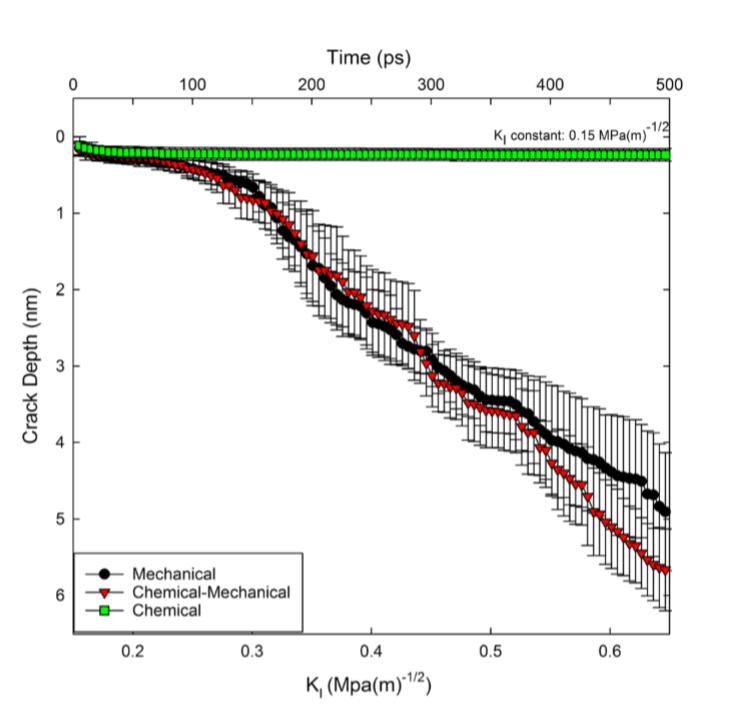
\includegraphics[width=11cm]{picture/crack_depth.PNG}
  \caption{Crack depth for silica systems under mechanical, chemical, and chemical-mechanical conditions.  Figure reproduced from~\protect\cite{chem_effects}}
  \label{crack_depth}
\end{figure}
\end{comment}

\begin{comment}
\begin{figure}[!b]
  \centering
  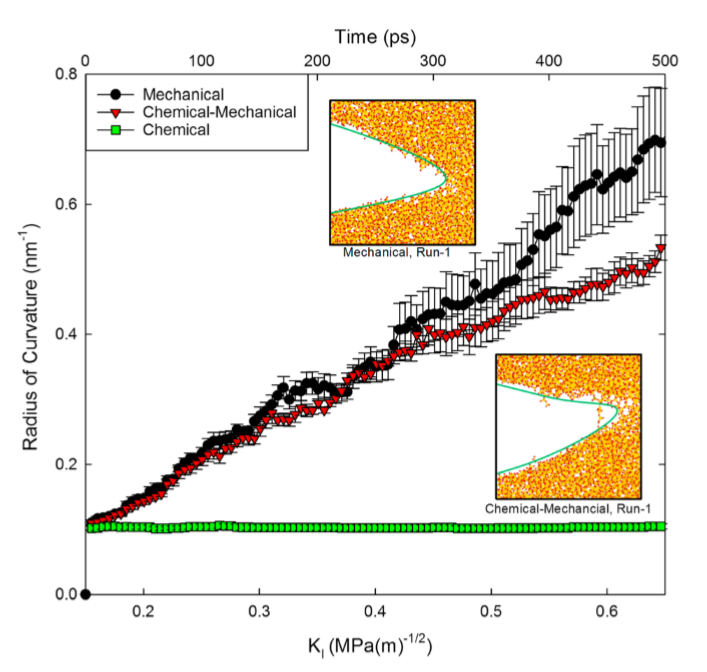
\includegraphics[width=11cm]{picture/crack_radius.PNG}
  \caption{Radius of curavture for silica systems under mechanical, chemical, and chemical-mechanical conditions. Figure reproduced from~\protect\cite{chem_effects}} 
  \label{crack_rad}
\end{figure}
\end{comment}



\begin{comment}
\begin{figure}[ht]
    \centering
    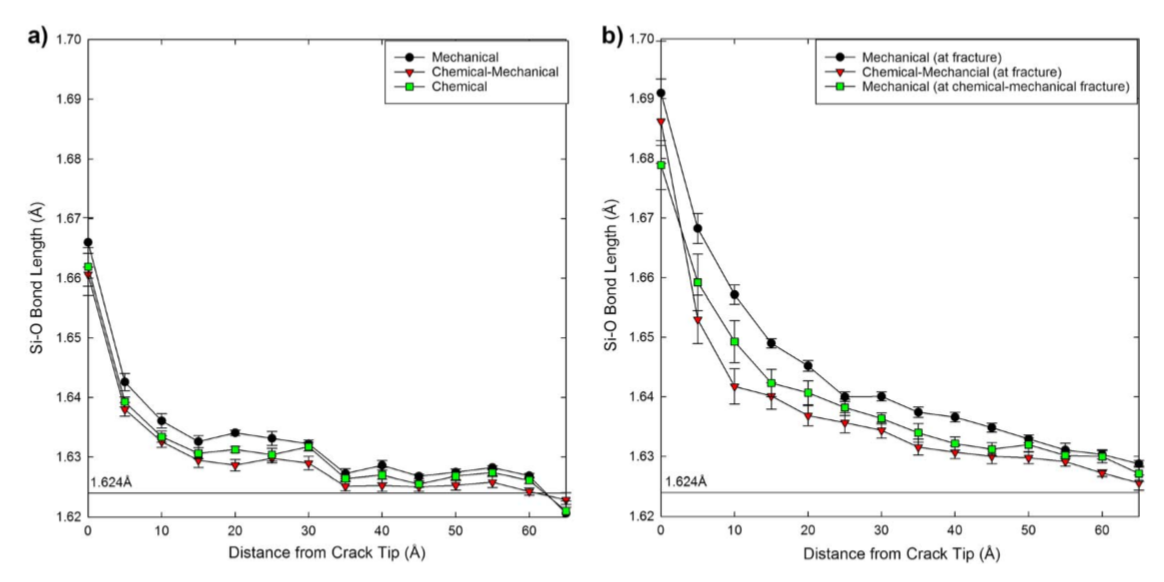
\includegraphics[width=10cm]{picture/AverageSiO.PNG}
    \caption{Average Si─O bond length based on distance from the crack tip at (a) initial conditions and (b) after loading.}
    \label{Average Si-O}
\end{figure}
\end{comment}


